\documentclass{beamer}
\mode<presentation> {
\usepackage{color}
\definecolor{bottomcolour}{rgb}{0.21,0.11,0.21}
\definecolor{middlecolour}{rgb}{0.21,0.11,0.21}
\setbeamercolor{structure}{fg=white}
\setbeamertemplate{frametitle}[default]%[center]
\setbeamercolor{normal text}{bg=black, fg=white}
\setbeamertemplate{background canvas}[vertical shading]
[bottom=bottomcolour, middle=middlecolour, top=black]
\setbeamertemplate{items}[circle]
\setbeamertemplate{navigation symbols}{} %no nav symbols
\setbeamercolor{block title}{use=structure,fg=white,bg=structure.fg!50!red!50!blue!100!green}
\setbeamercolor{block body}{parent=normal text,use=block title,bg=block title.bg!5!white!10!bg,fg=white}
\setbeamertemplate{navigation symbols}{}
}

\usepackage{graphicx} 
\usepackage{booktabs} 
\usepackage[utf8]{inputenc}  
\usepackage[T1]{fontenc}  
\usepackage{geometry}     
\usepackage[francais]{babel} 
\usepackage{eurosym}
\usepackage{verbatim}
\usepackage{ragged2e}
\justifying

%%%%%%%%%%%%%%%%%%%%%%%%%%%%%%%%%%%%%%%%%%%%%%%%%%%%%%%%%%%%%%%%
%% ccBeamer 0.1, 2007-07-02                                   %%
%% Written by Sebastian Pipping <webmaster@hartwork.org>      %%
%% ---------------------------------------------------------- %%
%% Licensed under Creative Commons Attribution-ShareAlike 3.0 %%
%% http://creativecommons.org/licenses/by-sa/3.0/             %%
%%%%%%%%%%%%%%%%%%%%%%%%%%%%%%%%%%%%%%%%%%%%%%%%%%%%%%%%%%%%%%%%


%% Images
\newcommand{\CcImageBy}[1]{%
	
\includegraphics[scale=#1]{creative_commons/cc_by_30.pdf}%
}
\newcommand{\CcImageCc}[1]{%
	
\includegraphics[scale=#1]{creative_commons/cc_cc_30.pdf}%
}
\newcommand{\CcImageDevNations}[1]{%
	
\includegraphics[scale=#1]{creative_commons/cc_dev_nations_30.pdf}%
}
\newcommand{\CcImageNc}[1]{%
	
\includegraphics[scale=#1]{creative_commons/cc_nc_30.pdf}%
}
\newcommand{\CcImageNd}[1]{%
	
\includegraphics[scale=#1]{creative_commons/cc_nd_30.pdf}%
}
\newcommand{\CcImagePd}[1]{%
	
\includegraphics[scale=#1]{creative_commons/cc_pd_30.pdf}%
}
\newcommand{\CcImageSa}[1]{%
	
\includegraphics[scale=#1]{creative_commons/cc_sa_30.pdf}%
}
\newcommand{\CcImageSampling}[1]{%
	
\includegraphics[scale=#1]{creative_commons/cc_sampling_30.pdf}%
}
\newcommand{\CcImageSamplingPlus}[1]{%
	
\includegraphics[scale=#1]{creative_commons/cc_sampling_plus_30.pdf}%
}


%% Groups
\newcommand{\CcGroupBy}[1]{% zoom
	\CcImageBy{#1}%
}
\newcommand{\CcGroupByNc}[2]{% zoom, gap
	\CcImageBy{#1}\hspace*{#2}\CcImageNc{#1}%
}
\newcommand{\CcGroupByNcNd}[2]{% zoom, gap
	\CcImageBy{#1}\hspace*{#2}\CcImageNc{#1}\hspace*{#2}\CcImageNd{#1}%
}
\newcommand{\CcGroupByNcSa}[2]{% zoom, gap
	\CcImageBy{#1}\hspace*{#2}\CcImageNc{#1}\hspace*{#2}\CcImageSa{#1}%
}
\newcommand{\CcGroupByNd}[2]{% zoom, gap
	\CcImageBy{#1}\hspace*{#2}\CcImageNd{#1}%
}
\newcommand{\CcGroupBySa}[2]{% zoom, gap
	\CcImageBy{#1}\hspace*{#2}\CcImageSa{#1}%
}
\newcommand{\CcGroupDevNations}[1]{% zoom
	\CcImageDevNations{#1}%
}
\newcommand{\CcGroupNcSampling}[2]{% zoom, gap
	\CcImageNc{#1}\hspace*{#2}\CcImageSampling{#1}%
}
\newcommand{\CcGroupPd}[1]{% zoom
	\CcImagePd{#1}%
}
\newcommand{\CcGroupSampling}[1]{% zoom
	\CcImageSampling{#1}%
}
\newcommand{\CcGroupSamplingPlus}[1]{% zoom
	\CcImageSamplingPlus{#1}%
}


%% Text
\newcommand{\CcLongnameBy}{Attribution}
\newcommand{\CcLongnameByNc}{Attribution-NonCommercial}
\newcommand{\CcLongnameByNcNd}{Attribution-NoDerivs}
\newcommand{\CcLongnameByNcSa}{Attribution-NonCommercial-ShareAlike}
\newcommand{\CcLongnameByNd}{Attribution-NoDerivs}
\newcommand{\CcLongnameBySa}{Attribution-ShareAlike}

\newcommand{\CcNote}[1]{% longname
	This work is licensed under the \textit{Creative Commons #1 3.0 License}.%
}


\title[]{
Les enjeux de la centralisation \\ des données personnelles \\ Sensibilisons aux risques,  \\proposons une alternative avec Framasoft} 
\author{Genma}
\date{Ubuntu Party - 30-31 mai 2015}
\begin{document}
\begin{frame}
	\titlepage
	\vfill
	\begin{center}
		\CcGroupByNcSa{0.83}{0.95ex}\\[2.5ex]
		{\tiny\CcNote{\CcLongnameByNcSa}}
		\vspace*{-2.5ex}
	\end{center}
\end{frame}

%----------------------------------------------------------------------------------------
\begin{frame}
\frametitle{
\includegraphics[scale=0.4]{./images/Genma.jpg} \ \ \  A propos de moi  }
\begin{columns}[c] 

\column{.55\textwidth} 
\textbf{Où me trouver sur Internet?}
\begin{itemize}
\item Le Blog de Genma : http://genma.free.fr
\item Twitter : http://twitter.com/genma
\end{itemize}

\textbf{Ce que je fais?}
\\ Plein de choses dont:
\begin{itemize}
\item Soutenir modestement Framasoft.
\end{itemize}

\column{.5\textwidth} 
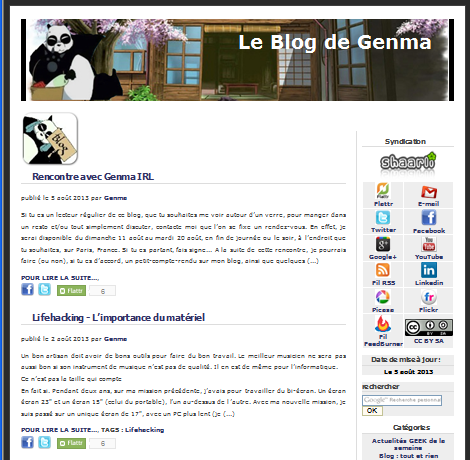
\includegraphics[width=5cm,height=5cm]{./images/blog.png} 
\end{columns}
\end{frame}


%----------------------------------------------------------------------------------------
\begin{frame}
\Huge{\centerline{Nous visons dans}}
\Huge{\centerline{un monde de plus en plus centralisé}}
\end{frame}


%------------------------------------------------
\begin{frame}
\frametitle{Enjeux}

\begin{block}{Les enjeux}
\justifying{
\begin{itemize}
\item Concentration des acteurs d’Internet autour de sillos
\item Une centralisation nuisible (frein à l'innovation)
\item  Les utilisateurs de ces services derniers ne contrôlent plus leur vie numérique
\end{itemize}
\begin{center}

\includegraphics[scale=0.3]{./images/fight.png}
\end{center}
}
\end{block}
Pius de détail sur \url{http://degooglisons-internet.org/}
\end{frame}

%------------------------------------------------
\begin{frame}
\frametitle{Les GAFAM}

\begin{block}{Les dangers}
\justifying{
Les services en ligne toujours plus centralisés de géants tentaculaires comme Google, Amazon, Facebook, Apple ou Microsoft (GAFAM) mettent en danger nos vies numériques.
\begin{itemize}
\item Espionnage
\item Vie privée
\item Centralisation
 \item Fermeture
\end{itemize}
\begin{center}

\includegraphics[scale=0.3]{./images/steve.png}\quad

\includegraphics[scale=0.3]{./images/legion.png}
\end{center}
}
\end{block}
Pius de détail sur \url{http://degooglisons-internet.org/}
\end{frame}


%----------------------------------------------------------------------------------------
\begin{frame}
\begin{center}
\Huge{Toutes ces informations \\ que l'on donne... }
\Huge{Volontairement...}
\Huge{ou pas}
\end{center}
\end{frame}

%------------------------------------------------
\begin{frame}
\frametitle{Rien qu'avec les services Google}

\begin{itemize}
\justifying{
\item Google Search
\item GMail 
\item Google Analytics 
\item Google Maps 
\item Smartphone Android 
\item Google Calendar 
\item Google Wallet 
\item Google Docs et Drive 
\item Google Chrome, navigateur 
\item Google Photos 
\item Youtube 
\item ...
}
\end{itemize}

\end{frame}


%------------------------------------------------
\begin{frame}
\frametitle{Les applications pour Smartphone}
\begin{block}{75 \% des applis mobiles collectent des données personnelles}
\justifying{
Selon une étude réalisée par la CNIL et ses homologues européennes, avec l'examen de plus de 1200 applications mobiles,
 les trois quarts des applis installées sur les smartphones collectent des données personnelles, et la plupart le font avec une information insuffissante du consommateur.
}
Source \url{http://www.numerama.com}
\end{block}
Est-il normal qu'une application lampe de poche est besoin d'accéder au carnet d'adresses?
\end{frame}

%----------------------------------------------------------------------------------------
\begin{frame}
\begin{center}
\Huge{Et ce sans parler de l'arrivée des objets connectés, \\ du tracking Internet... }
\end{center}
\end{frame}


%----------------------------------------------------------------------------------------
\begin{frame}
\begin{center}
\Huge{Conséquences de l'usage de toutes ces données }
\end{center}
\end{frame}

%----------------------------------------------------------------------------------------
\begin{frame}
\begin{center}
\Huge{A une échelle BigData}
\end{center}
\end{frame}

%------------------------------------------------
\begin{frame}
\frametitle{GoogleFlu et Google trends}
\begin{block}{Présentation de Google Flux sur leur site}
\begin{itemize}
\justifying{
\item Nous avons remarqué que certains termes de recherche étaient des indicateurs efficaces de la propagation de la grippe. Google Flu rassemble donc des données de recherche Google pour fournir une estimation quasiment en temps réel de cette propagation à l'échelle mondiale. \url{http://www.google.org/flutrends/}
\item On peut aussi voir les recherches temps réels, par mot clef, pays... \url{https://www.google.com/trends/}
}
\end{itemize}
\end{block}
\justifying{
Tout cela ne me laisse pas indifférent quand à \textbf{ la puissance de Google}. Et vous?
}
\end{frame}

%----------------------------------------------------------------------------------------
\begin{frame}
\Huge{\centerline{A l'échelle de l'individu...}}
\end{frame}


%----------------------------------------------------------------------------------------
\begin{frame}
\begin{center}
\Huge{Sur Internet, si c'est gratuit, c'est vous le produit }
\end{center}
\end{frame}
%----------------------------------------------------------------------------------------
\begin{frame}
\frametitle{Qu'est-ce que le pistage ?}
\begin{block}{Le pistage sur Internet}
\begin{itemize}
\justifying{
\item Le pistage est un terme qui comprend des méthodes aussi nombreuses et variées que les sites web, les annonceurs et d'autres utilisent pour connaître vos habitudes de navigation sur le Web. 
\item  Cela comprend des informations sur les sites que vous visitez, les choses que vous aimez, n'aimez pas et achetez. 
\item Ils utilisent souvent ces données pour afficher des pubs, des produits ou services spécialement ciblés pour vous. 
}
\end{itemize}
\end{block}
\end{frame}

%----------------------------------------------------------------------------------------
\begin{frame}
\frametitle{Comment est-on tracké?}

\justifying{
\begin{block}{Toutes les publicités nous espionnent}
\begin{itemize}
\item Le bouton Like de Facebook : il permet à FaceBook de savoir que vous avez visité ce site, même si vous n'avez pas cliqué sur ce bouton.
\item Même si vous vous êtes correctement déconnecté de Facebook.
\item De même pour le bouton le +1 de Google, les scripts de Google Analytics, 
\item Tous les publicité, Amazon...
\end{itemize}
\end{block}
}
\begin{center}

\includegraphics[scale=0.3] {./images/Facebook_like.png}
\end{center}

\end{frame}

%----------------------------------------------------------------------------------------
\begin{frame}
\begin{center}
\Huge{Et tout ceci est lié à \\ la Centralisation d'Internet}
\end{center}
\end{frame}

%----------------------------------------------------------------------------------------
\begin{frame}
\Huge{\centerline{Existe-t-il une solution?}}
\end{frame}


%----------------------------------------------------------------------------------------
\begin{frame}
\Huge{\centerline{Framasoft}}
\Huge{\centerline{(une solution parmi d'autres)}}
\begin{center}

\includegraphics[scale=0.6]{./images/pingouinVolantRefait.jpg}
\end{center}
\end{frame}


%------------------------------------------------
\begin{frame}
\frametitle{Framasoft c'est quoi?}

\begin{block}{Présentation}
\justifying{
Framasoft est une association francophone de promotion et diffusion des logiciels libres. C'est aussi
\begin{itemize}
\item Un réseau dédié à la promotion du « libre » en général et du logiciel libre en particulier.
\item De nombreux services et projets innovants mis librement à disposition du grand public.
\item Une communauté de bénévoles soutenue par une association d’intérêt général.
\item Une invitation à bâtir ensemble un monde de partage et de coopération.
\end{itemize}
}
\end{block}
Plus de détail sur \url{http://www.framasoft.org}
\end{frame}

%------------------------------------------------
\begin{frame}
\frametitle{Framasoft en quelques chiffres}

\begin{block}{Des chiffres}
\justifying{
\begin{itemize}
\item 12 ans d’existence, 1 association et 2 permanents
\item 1 réseau, 1 000 000 visites par mois
\item 20 projets, 15 serveurs, 50 noms de domaine et 30 CMS déployés
\item 10 000 abonnés Twitter
\item 1 600 logiciels libres dans notre annuaire
\item 200 000 logiciels installés via Framapack
\item 750 000 clés framakeys téléchargées
\item 4 000 000 clés diffusées
\end{itemize}
}
\end{block}
Plus de détail sur \url{http://www.framasoft.org}
\end{frame}

%----------------------------------------------------------------------------------------
\begin{frame}
\Huge{\centerline{Framasoft et la dégooglisation}}
\begin{center}

\includegraphics[scale=0.6]{./images/cloud.jpg}
\end{center}
\end{frame}

\begin{frame}
\begin{center}
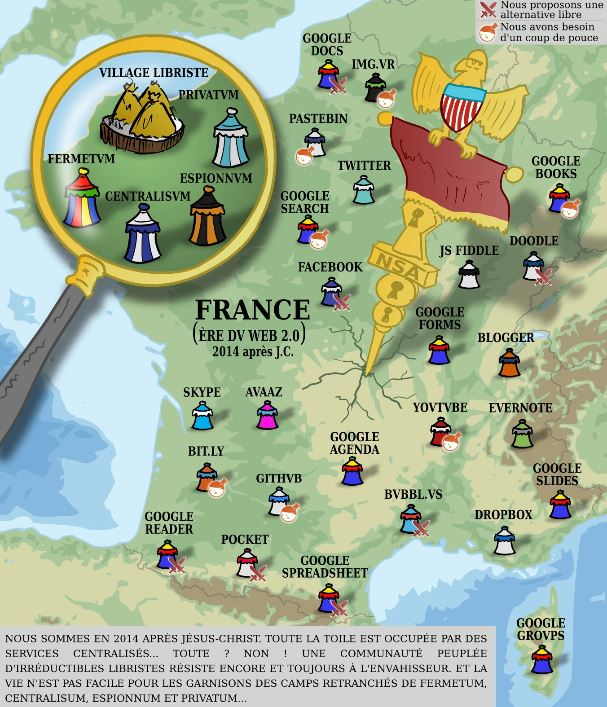
\includegraphics[scale=0.5]{./images/DegooglisonsInternet.jpg}
\end{center}
\end{frame}
%------------------------------------------------
\begin{frame}
\frametitle{Dégooglisons Internet}

\begin{block}{Framasoft lance une campagne d’envergure : Dégooglisons Internet. }
\justifying{
Après avoir mis en place Framapad, Framadate, Framindmap, Framanews et le petit dernier Framabag, il était temps de passer à la vitesse supérieure en annonçant la mise en place de plus de services L.E.D.S. (Libres, Éthiques, Décentralisés et Solidaires). 
\\~\\L’annonce s’est donc accompagnée de l’ouverture d’un nouveau pod Diaspora* pour les francophones soucieux de leur vie privée : la Framasphère.
}
\end{block}
\end{frame}

%------------------------------------------------
\begin{frame}
\frametitle{Dégooglisons Internet}

\begin{block}{L'objectif}
\justifying{
Les logiciels libres, de par leur nature ouverte, sont les seuls à vraiment garantir le respect de votre vie privée.
\\~\\
Il faut donc installer, face à chaque service propriétaire, un service hébergé par les soins de Framasoft. 
\\~\\L’association s’inscrit dans un contexte d’ouverture en encourageant les projets qui participeront à cet effort d’émancipation des « grands de l’Internet ».
}
\end{block}
Plus de détail sur \url{http://degooglisons-internet.org/}
\end{frame}


%------------------------------------------------
\begin{frame}
\frametitle{Enjeux}

\begin{block}{Les enjeux}
\justifying{
\begin{itemize}
\item Concentration des acteurs d’Internet autour de sillos
\item Une centralisation nuisible (frein à l'innovation)
\item  Les utilisateurs de ces services derniers ne contrôlent plus leur vie numérique
\end{itemize}
\begin{center}

\includegraphics[scale=0.3]{./images/fight.png}
\end{center}
}
\end{block}
Pius de détail sur \url{http://degooglisons-internet.org/}
\end{frame}

%------------------------------------------------
\begin{frame}
\frametitle{Dangers}

\begin{block}{Les dangers}
\justifying{
Les services en ligne toujours plus centralisés de géants tentaculaires comme Google, Amazon, Facebook, Apple ou Microsoft (GAFAM) mettent en danger nos vies numériques.
\begin{itemize}
\item Espionnage
\item Vie privée
\item Centralisation
 \item Fermeture
\end{itemize}
\begin{center}

\includegraphics[scale=0.3]{./images/steve.png}\quad

\includegraphics[scale=0.3]{./images/legion.png}
\end{center}
}
\end{block}
Pius de détail sur \url{http://degooglisons-internet.org/}
\end{frame}

%------------------------------------------------
\begin{frame}
\frametitle{Les propositions de Framasoft}

\begin{block}{Ce que Framasoft propose}
\justifying{
Framasoft souhaite faire face à ces dangers menaçant nos vies numériques en proposant des services
\begin{itemize}
\item  libres,
\item éthiques, 
\item décentralisés 
\item et solidaires.
\end{itemize}
\begin{center}

\includegraphics[scale=0.3]{./images/potion.png}
\end{center}
}
\end{block}
Plus de détail sur \url{http://degooglisons-internet.org/}
\end{frame}

%------------------------------------------------
\begin{frame}
\frametitle{Concrètement, ce que fait Framasoft}

\begin{block}{Concrètement}
Le projet « Dégooglisons Internet » - qui ne concerne d'ailleurs pas que Google - consiste à proposer des services alternatifs face à un maximum de services que nous évaluons comme menaçants pour nos vies numériques.
\justifying{
\begin{itemize}
\item Des services sont libres, gratuits, ouverts à tous (dans la limite de nos capacités techniques et financières),
\item Promotion de l'auto-hébergement, 
\item Proposer une alternative.
\end{itemize}
}
\end{block}
Plus de détail sur \url{http://degooglisons-internet.org/}
\end{frame}

%----------------------------------------------------------------------------------------
\begin{frame}
\Huge{\centerline{Les services "cloud" de Framasoft}}
\begin{center}

\includegraphics[scale=0.6]{./images/Framacloud.jpg}
\end{center}
\end{frame}
%------------------------------------------------

\begin{frame}
\begin{center}
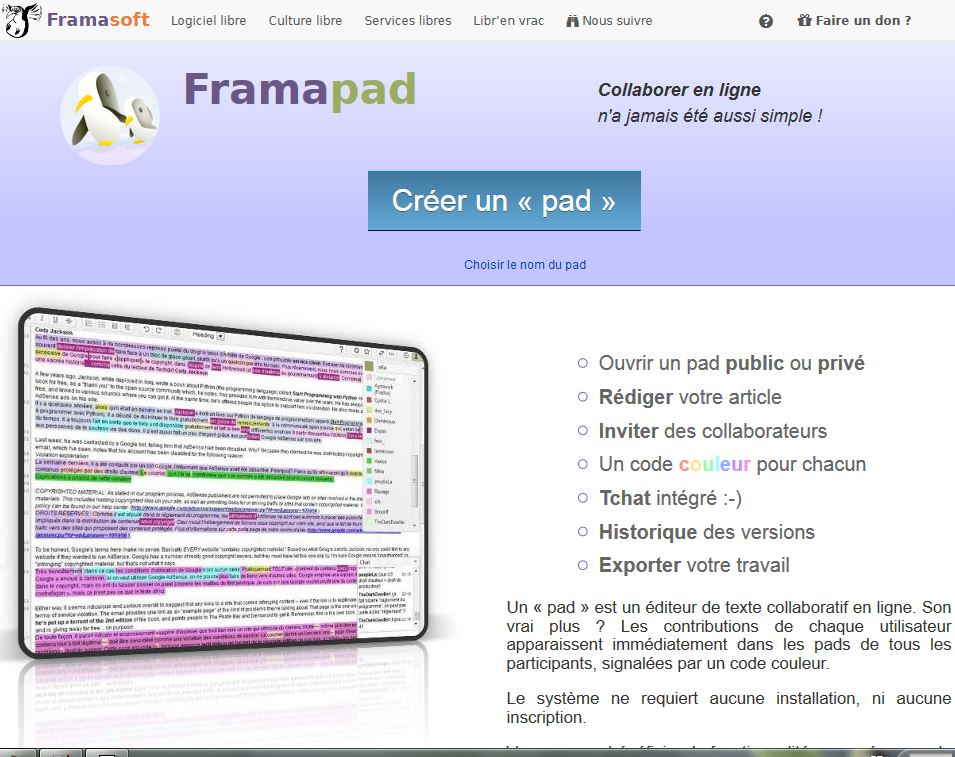
\includegraphics[scale=0.5]{./images/Framapad.jpg}
\end{center}
\end{frame}

\begin{frame}
\begin{center}
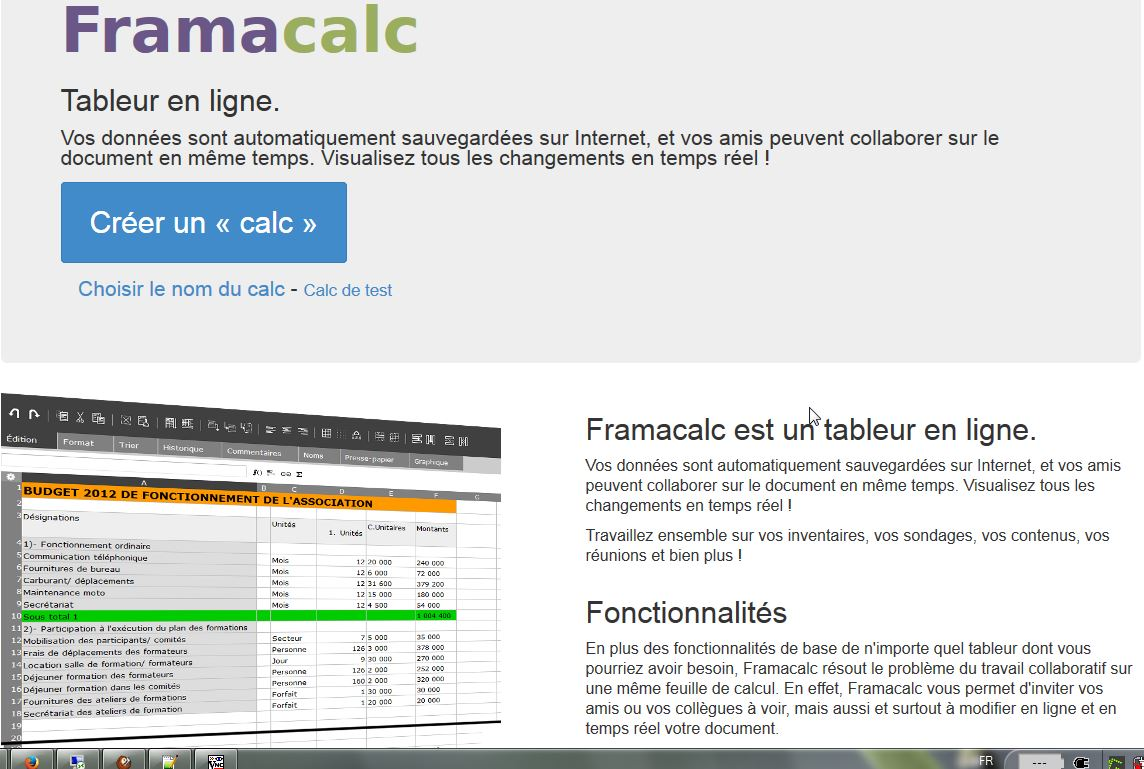
\includegraphics[scale=0.5]{./images/FramaCalc.jpg}
\end{center}
\end{frame}

\begin{frame}
\begin{center}
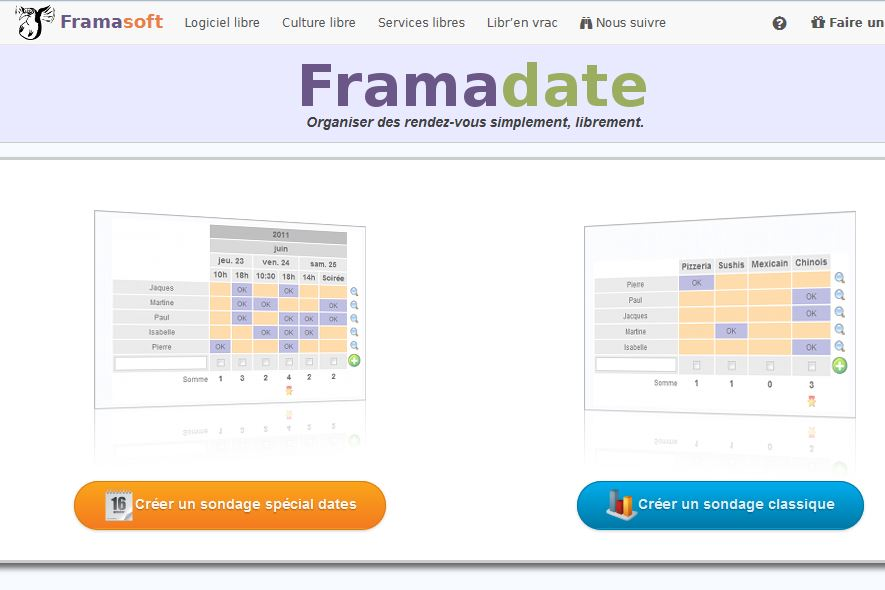
\includegraphics[scale=0.5]{./images/Framadate.jpg}
\end{center}
\end{frame}

\begin{frame}
\begin{center}
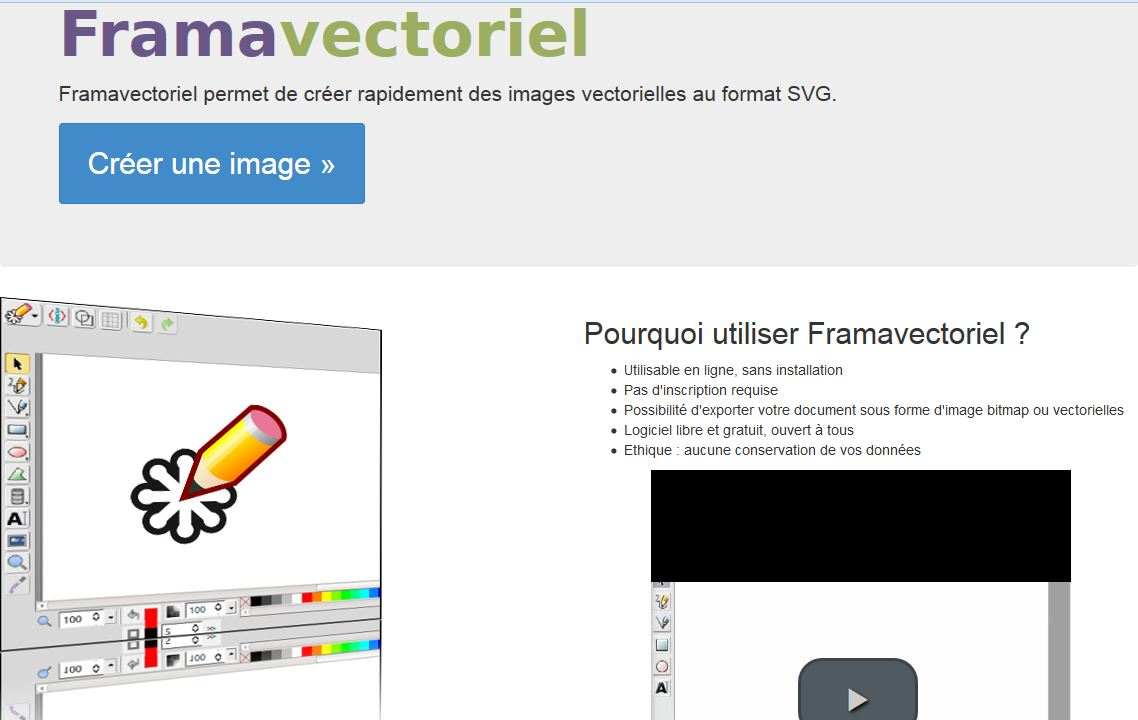
\includegraphics[scale=0.5]{./images/Framavectoriel.jpg}
\end{center}
\end{frame}

\begin{frame}
\begin{center}
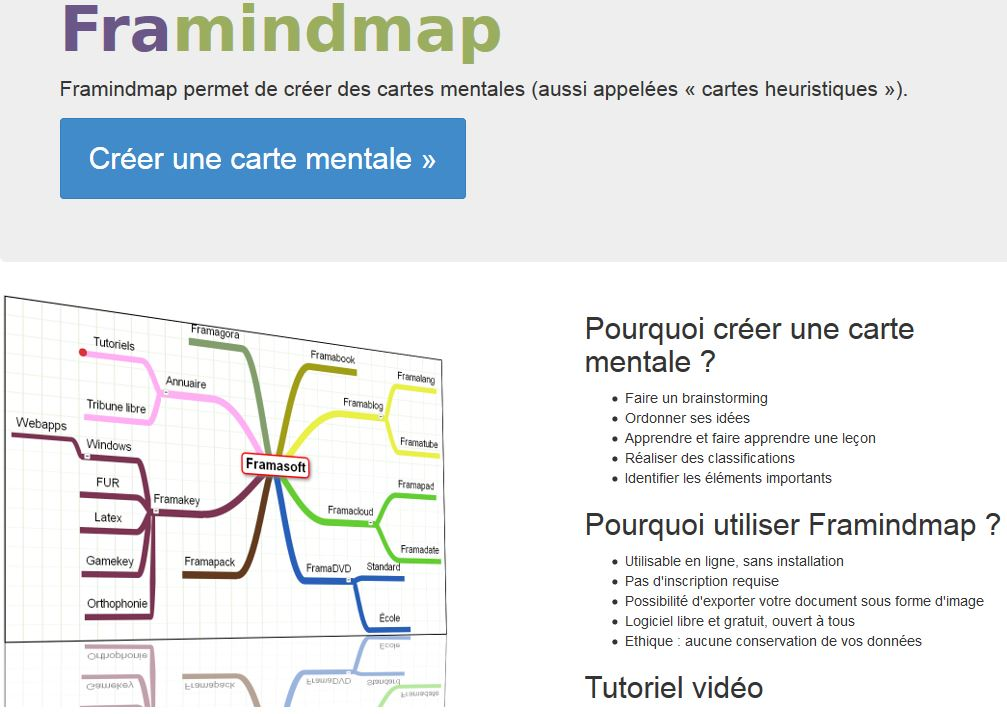
\includegraphics[scale=0.5]{./images/Framindmap.jpg}
\end{center}
\end{frame}

\begin{frame}
\begin{center}
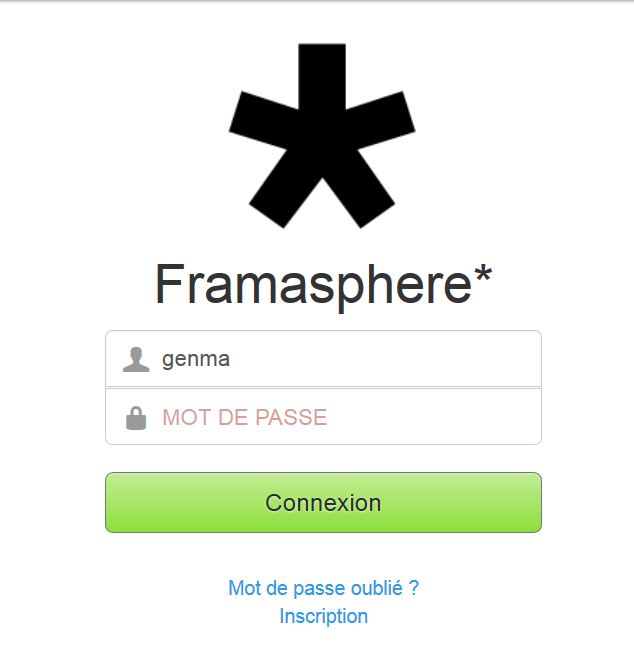
\includegraphics[scale=0.5]{./images/Framasphere.jpg}
\end{center}
\end{frame}

\begin{frame}
\begin{center}
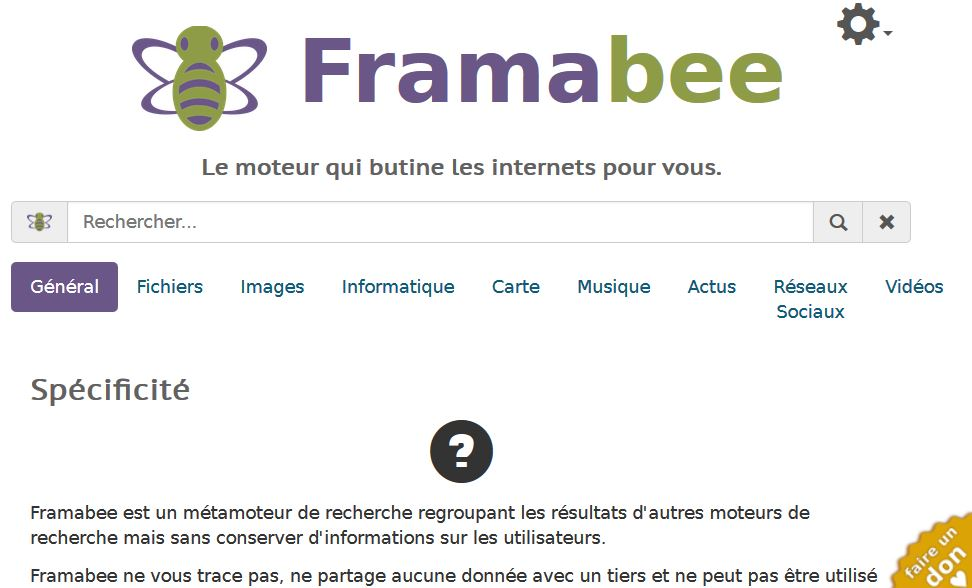
\includegraphics[scale=0.5]{./images/Framabee.jpg}
\end{center}
\end{frame}


\begin{frame}
\Huge{\centerline{Et d'autres à l'avenir...}}
\end{frame}

\begin{frame}
\begin{center}
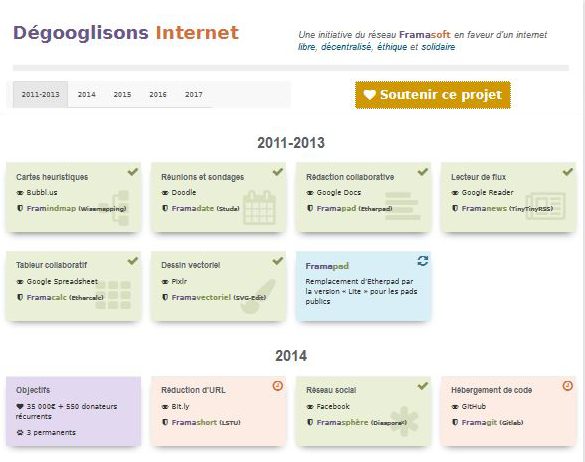
\includegraphics[scale=0.5]{./images/Roadmap.jpg}
\end{center}
\end{frame}

%----------------------------------------------------------------------------------------
\begin{frame}
\Huge{\centerline{C'est gratuit...}}
\Huge{\centerline{...mais ce n'est plus nous le produit!}}
\end{frame}
%------------------------------------------------

%----------------------------------------------------------------------------------------
\begin{frame}
\begin{center}
\Huge{Soutenons Framasoft \\ dans cette initiative}
\end{center}
\end{frame}
%------------------------------------------------

\begin{frame}
\begin{center}
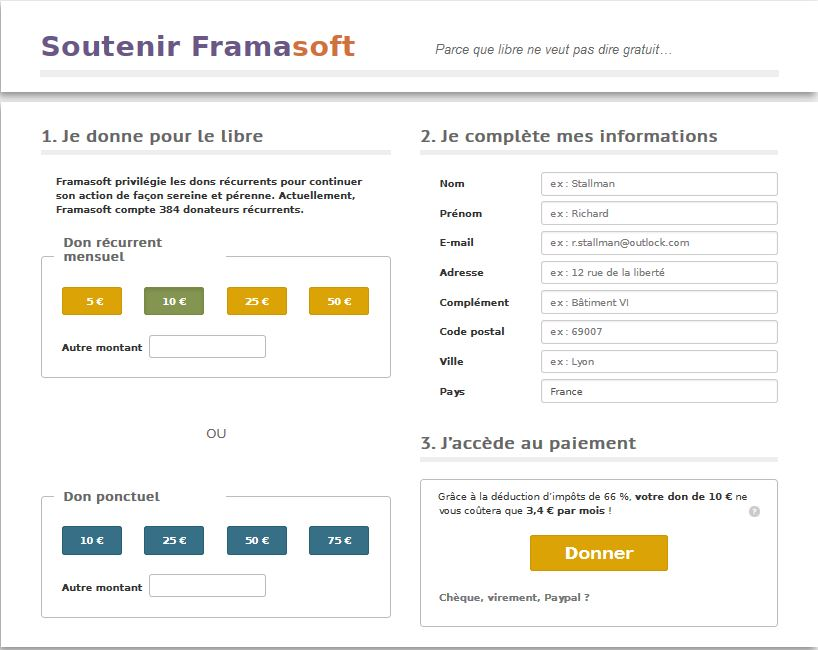
\includegraphics[scale=0.5]{./images/Soutien01.jpg}
\end{center}
\end{frame}

%------------------------------------------------
\begin{frame}
\frametitle{Pourquoi soutenir Framasoft}

\begin{block}{6 bonnes raisons de nous soutenir}
\justifying{
\begin{itemize}
\item Parce que l’enfermement, c’est maintenant.
\item Pour plus d’alternatives libres.
\item Parce que les gentils, c’est nous !
\item Pour décider où vont vos impôts (avec défiscalisation).
\item Parce que l’économie du don rend indépendant.
\item Pour changer le monde ensemble.
\end{itemize}
}
\end{block}
\end{frame}


%------------------------------------------------
\begin{frame}
\frametitle{Framasoft est transparent sur l'usage des dons}

\begin{center}
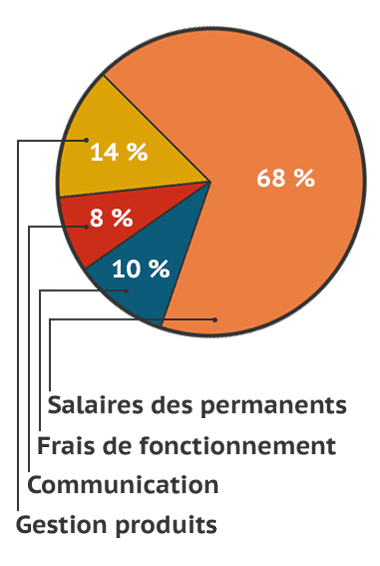
\includegraphics[scale=0.3]{./images/graphique.jpg}
\\~\\
\url{https://soutenir.framasoft.org/}
\end{center}
\end{frame}


%----------------------------------------------------------------------------------------
\begin{frame}
\Huge{\centerline{Participer à l'aventure Framasoft}}
\end{frame}
%------------------------------------------------

%------------------------------------------------
\begin{frame}
\frametitle{Participer à Framasoft}

\begin{block}{Comment participer?}
\justifying{
En participer aux projets existants :
\begin{itemize}
\item Support technique (administration, développement)
\item Traduction, relecture...
\item Communication, graphisme...
\end{itemize}
Ou en proposant un nouveau projet!
}
\\~\\
\url{http://framalistes.org/sympa/lists}
\end{block}
\end{frame}

%----------------------------------------------------------------------------------------
\begin{frame}
\Huge{\centerline{Merci de votre attention.}}
\Huge{\centerline{Place aux questions. Débattons...}}
\begin{center}

\includegraphics[scale=0.2]{./images/chat.jpg}
\end{center}

\end{frame}

\end{document}
